\documentclass[tikz,border=2pt]{standalone}
\usepackage{times}
\usepackage{amsmath}
\usepackage{pgfplots}
\pgfplotsset{compat=1.16}
\begin{document}
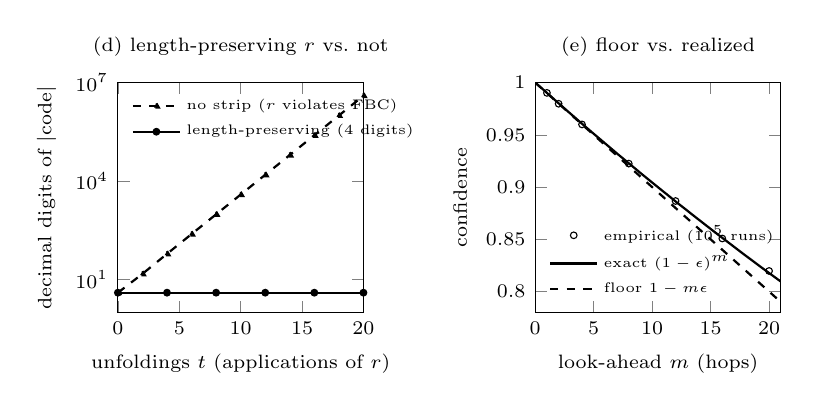
\begin{tikzpicture}
% (d) code length under t unfoldings: with vs without the length-preserving discipline
\begin{axis}[
  width=4.7cm, height=4.5cm, font=\scriptsize,
  xlabel={unfoldings $t$ (applications of $r$)}, ylabel={decimal digits of $|\text{code}|$},
  ymode=log, xmin=0, xmax=20, ymin=1, ymax=1e7,
  title={\scriptsize (d) length-preserving $r$ vs.\ not},
  legend style={font=\tiny, at={(0.02,0.98)}, anchor=north west, draw=none, fill=none},
  legend cell align=left,
]
% no-strip: digits = log10(length); length ~ 2^(2^t): doubly exponential
\addplot[mark=triangle*, mark size=1pt, thick, dashed] coordinates {(0,4)(2,15)(4,61)(6,244)(8,975)(10,3898)(12,15593)(14,62372)(16,249486)(18,997945)(20,3991780)};
\addlegendentry{no strip ($r$ violates FBC)}
% compliant: constant 3200 -> 4 digits
\addplot[mark=*, mark size=1pt, thick] coordinates {(0,4)(4,4)(8,4)(12,4)(16,4)(20,4)};
\addlegendentry{length-preserving (4 digits)}
\end{axis}
% (e) confidence floor vs realized confidence
\begin{scope}[xshift=5.3cm]
\begin{axis}[
  width=4.7cm, height=4.5cm, font=\scriptsize,
  xlabel={look-ahead $m$ (hops)}, ylabel={confidence},
  ymin=0.78, ymax=1.0, xmin=0, xmax=21,
  title={\scriptsize (e) floor vs.\ realized},
  legend style={font=\tiny, at={(0.02,0.02)}, anchor=south west, draw=none, fill=none},
  legend cell align=left,
]
\addplot[only marks, mark=o, mark size=1.2pt] coordinates {(1,0.9902)(2,0.9798)(4,0.9600)(8,0.9225)(12,0.8867)(16,0.8508)(20,0.8197)};
\addlegendentry{empirical ($10^5$ runs)}
\addplot[domain=0:21, thick, samples=40] {(1-0.01)^x};
\addlegendentry{exact $(1-\epsilon)^m$}
\addplot[domain=0:21, thick, dashed] {1-0.01*x};
\addlegendentry{floor $1-m\epsilon$}
\end{axis}
\end{scope}
\end{tikzpicture}
\end{document}
